\documentclass[11pt,oneside]{book}
\usepackage[backend=biber,natbib=true,style=alphabetic,maxbibnames=10]{biblatex}
\addbibresource{/home/nqbh/reference/bib.bib}
\usepackage[utf8]{vietnam}
\usepackage{tocloft}
\renewcommand{\cftsecleader}{\cftdotfill{\cftdotsep}}
\usepackage[colorlinks=true,linkcolor=blue,urlcolor=red,citecolor=magenta]{hyperref}
\usepackage{amsmath,amssymb,amsthm,chemfig,fancyhdr,float,graphicx,mathtools,multicol,soul}
\usepackage[version=4]{mhchem}
\allowdisplaybreaks
\newtheorem{assumption}{Assumption}
\newtheorem{baitoan}{Bài toán}
\newtheorem{cauhoi}{Câu hỏi}
\newtheorem{conjecture}{Conjecture}
\newtheorem{corollary}{Corollary}
\newtheorem{dangtoan}{Dạng toán}
\newtheorem{definition}{Definition}
\newtheorem{dinhly}{Định lý}
\newtheorem{dinhnghia}{Định nghĩa}
\newtheorem{example}{Example}
\newtheorem{goal}{Goal}
\newtheorem{ghichu}{Ghi chú}
\newtheorem{hequa}{Hệ quả}
\newtheorem{hypothesis}{Hypothesis}
\newtheorem{lemma}{Lemma}
\newtheorem{luuy}{Lưu ý}
\newtheorem{muctieu}{Mục tiêu}
\newtheorem{nhanxet}{Nhận xét}
\newtheorem{notation}{Notation}
\newtheorem{note}{Note}
\newtheorem{principle}{Principle}
\newtheorem{problem}{Problem}
\newtheorem{proposition}{Proposition}
\newtheorem{question}{Question}
\newtheorem{quyuoc}{Quy ước}
\newtheorem{remark}{Remark}
\newtheorem{theorem}{Theorem}
\newtheorem{vidu}{Ví dụ}
\usepackage[margin=2cm,footskip=1cm]{geometry}
\DeclareRobustCommand{\divby}{%
	\mathrel{\vbox{\baselineskip.65ex\lineskiplimit0pt\hbox{.}\hbox{.}\hbox{.}}}%
}

\title{Dạy Trẻ Vùng Quê}
%\title{Some Topics in Elementary STEM \textit{\&} Beyond:\\A Personal, Psychological, \textit{\&} Philosophical Perspective\\\vspace{1cm}\textsf{\Large Vài Vấn Đề Trong STEM Sơ Cấp \& Xa Hơn Thế:\\1 Góc Nhìn Cá Nhân, Tâm Lý Học, \& Triết Học.}}
\author{Nguyễn Quản Bá Hồng\footnote{A Scientist- \& Creative Artist Wannabe. e-mail: {\sf nguyenquanbahong@gmail.com}, website: \url{https://nqbh.github.io}, Ben Tre City, Vietnam.}}
\date{\today}

\begin{document}
\maketitle
\begin{quotation}
	\textit{``In this world, is the destiny of mankind controlled by some transcendental entity or law? Is it like the hand of God hovering above? At least it is true that man has no control, even over his own will. Man takes up the sword in order to shield the small wound in his heart sustained in a far-off time beyond remembrance. Man wields the sword so that he may die smiling in some far-off time beyond perception.''} -- \textsc{Kentaro Miura}, \textit{Berserk}, Vol. 1
	\begin{figure}[H]
		\centering
		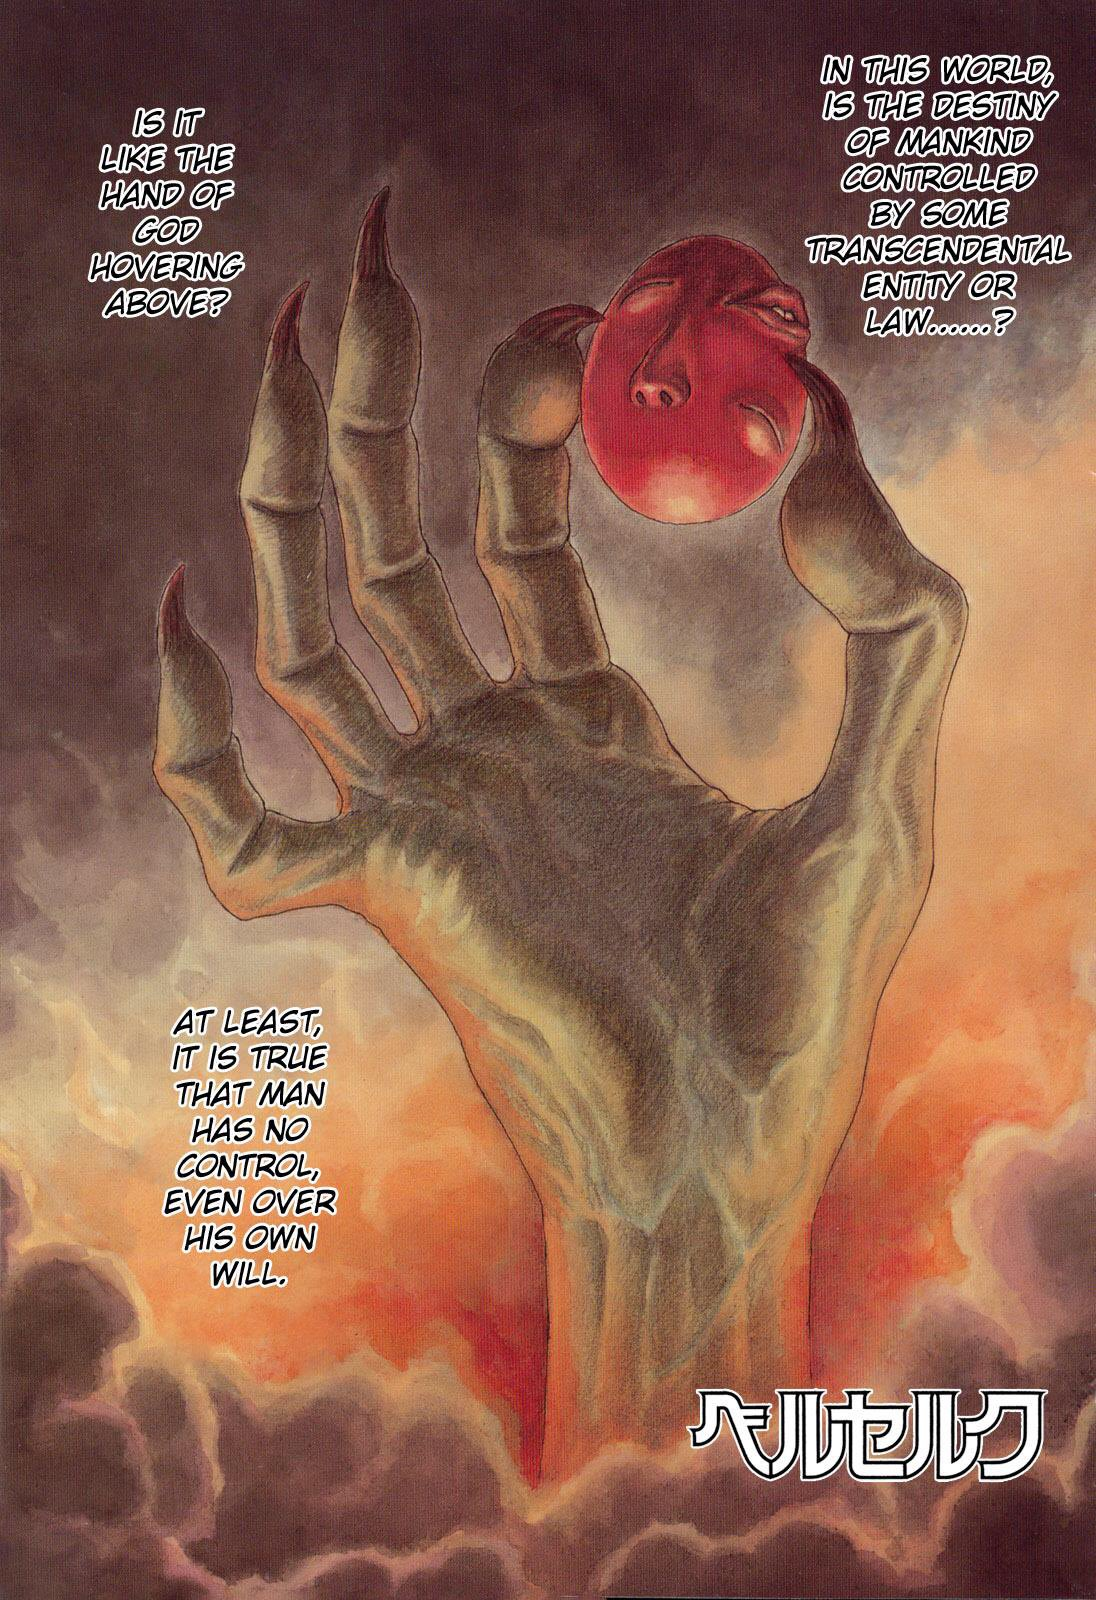
\includegraphics[scale=.15]{Berserk_behelit_color}
		\caption{Berserk, The Hand of God \textit{\&} Behelit.}
	\end{figure}	
	\textit{``Providence may guide a man to meet 1 specific person, even if such guidance eventually leads him to darkness. Man simply cannot forsake the beauty of his own chosen path. When will man learn a way to control his soul?''} – \textsc{Kentaro Miura}, \textit{Berserk}
\end{quotation}
%\hrule
%\begin{multicols}{2}
%	\textit{``What are you doing actually?''} ``I am writing a book.'' \textit{``About what?''} ``I don't know yet.'' \textit{``Huh? You want to write a book but you don't know specifically what to write yet? How can that be?''} ``Everything starts with a sheer will to write, I suppose.'' \textit{``What a joke!''} ``Yeah, let my innocent Infinite Jest \footnote{\textit{Infinite Jest} is the name of a book written by \textsc{David Foster Wallace}, a genius, suicide in ??.} begin.''
%	\columnbreak
%	
%	\textit{``Thực sự là mày đang làm gì vậy?''} ``Tui đang viết 1 cuốn sách.'' \textit{``Về cái gì?''} ``Tui cũng chưa biết nữa.'' \textit{``Hả, mày muốn viết 1 cuốn sách nhưng mày chưa biết viết cụ thể về cái gì? Sao có thể được?''} ``Mọi thứ đều bắt đầu với 1 quyết tâm để viết, tui giả dụ vậy.'' \textit{``Đúng là 1 trò hề!''} ``Ừa, cứ để Trò Hề Vô Hạn nhưng vô hại này bắt đầu.''	
%\end{multicols}
%\hrule
%\noindent
%\begin{verbatim}
%	nqbh@nqbh-mind:~$ reboot
%\end{verbatim}
\chapter{Nghề Chăn Báo}
Tui dự định viết ghi chú này từ cuối năm 2020, cho bản thân là chính (self-growth -- phát triển cá nhân\footnote{Xem Wikipedia{\tt/}phát triển cá nhân.}), chứ tui không viết \textit{vì ai đó hoặc vì muốn tốt cho người khác}, hoặc để thể hiện hoặc sẽ viết vì mục đích thể hiện cả. Tui đã từng nhiều lần làm thế rồi, nên bây giờ \& từ giờ trở đi tui sẽ không làm thế, bởi tui thấy nó thật vô nghĩa \& tui biết vậy. Đơn giản là nếu chỉ để thể hiện như 1 con ngựa non háo đá, tui sẽ nhanh chóng nhận ra mình ngu dốt, thiếu chín chắn, thùng rỗng kêu to cỡ nào rồi lại tự nhục, rồi xóa, rồi kiếm 1 cái gì khác để thể hiện, rồi lại tự nhận thức được rồi nhục, rồi lại tự xóa. Cái vòng thể hiện-nhục-thể hiện-nhục lẩn quẩn cứ lặp đi lặp lại nếu tui mãi không phát triển nhận thức, nên tui sẽ cắt nó ngay từ đầu. Trong hơn 3 năm qua, kể từ cuối năm 2020 -- lần nói chuyện cuối cùng với thầy Quí - thầy dạy Toán cấp 3 của tui, đến nay, đầu năm 2024, có nhiều điều đã thay đổi trong cách nhìn của tui về hành vi, mục đích, các lựa chọn của bản thân \& quan trọng hơn là những cách nhìn mới về cuộc sống. Có thể tui cũng chỉ đang trải qua những giai đoạn trưởng thành bên trong mà nhiều người bạn hoặc nhiều em ít tuổi hơn tui đã trải qua từ kiếp nào so với 1 đứa trưởng thành về cảm xúc vừa chậm vừa trễ như tui, nhưng cũng đáng để ghi lại.

Ban đầu tui định đặt tên cho ghi chú này là \textit{``Some Topics on Elementary STEM \& Beyond: A Personal, Psychological \& Philosophical Perspective: Vài Vấn Đề Trong STEM Sơ Cấp \& Xa Hơn Thế: 1 Góc Nhìn Cá Nhân, Tâm Lý Học, \& Triết Học.''} nhưng đọc tới đọc lui thấy nó hào nhoáng kiểu tởm quá xá, chưa kể tựa đọc nghe cọp mà nội dung như hạch thì lại áp lực mà phải sửa văn cho hay, cho phù hợp. Thế là tui đọc sách để kiếm 1 cái tên đơn giản để phù hợp. Có vẻ cuốn sách gần nhất với nội dung mà tui định viết là cuốn \textit{Bắt Trẻ Đồng Xanh} \cite{Salinger_btdx} của {\sc Jerome David Salinger} (tựa gốc tiếng anh: {\it The Catcher In The Rye} \cite{Salinger_catcher_in_rye}). Tui hay nói đùa với mấy đứa học tui là để làm nghề chăn báo dưới quê thì phải đọc quyển này để hiểu rõ tâm lý chán chường, quậy phá, nông nổi của lũ trẻ, đặc biệt là lũ báo non. Nhưng nếu tui bắt chước theo mà đặt tên cho bài viết của tui là ``Bắt Trẻ Đồng Quê'' hoặc ``Bắt Trẻ Vùng Quê'' thì nghe như pedophile\footnote{Vài thầy giáo trường cấp 2 cũ của tui có sở thích kê sát người rồi hửi học sinh nữ. Vài ông còn làm cho nhiều học sinh nữ có bầu nên tui tuyệt đối tránh điều này. Tui chỉ mê phụ nữ có tuổi hơn kém tui 3 đơn vị, i.e., phải thỏa mãn điều ràng buộc $\rm|age(I) - age(her)|\le3\land\min\{age(I),age(her)\}\ge18$.}, hay Child Trafficking, không khéo lại vô tù nên chả ổn tí nào. Thành ra ``Dạy Trẻ Vùng Quê'' là ổn nhất, ``Dạy Trẻ Đồng Quê'' không hợp lắm vì ``Đồng Quê'' áp chỉ sự nghèo khó nhưng chất phác của dân quê, nhưng giờ thì nhiều nhà ở quê giàu quá nên áp vào lại sai be bét. Cái chính vẫn là mớ tâm lý bất ổn, rối nùi như cái mớ bòng bong, với cách hành xử của bọn trẻ Gen Z với mọi người xung quanh ở quê trong cái thời đại mà mọi công nghệ tiên tiến đều được đáp ứng đủ phần nào để lũ trẻ thoát khỏi cái tuổi thơ rừng rú của tui để ham học, nhưng lại tối ngày đi stalk acc online người khác, xem phim heo, \& đủ thứ chuyện hại não khác làm cho chúng sau này chả tập trung làm được điều gì cho đâu vào đấy. Chính là ở chỗ ấy: \textit{tập trung để làm 1 cái gì đó đâu vào đấy}. Cái ấy mới quan trọng cho lũ nhỏ, không phải tiền bạc dư thừa để mua laptop hoặc nguyên dàn PC gaming siêu xịn để cả lũ con trai lớp 4, 5 túm tụm xem phim heo \& thuộc lòng nhiều tên diễn viên người lớn hơn các ông thầy cô đơn của chúng, trong khi không nhớ nổi 1 công thức toán hoặc giải 1 phương trình đơn giản. Đấy lại là nỗi đau thứ 2 của các ông thầy.

Nói thật tui chả biết phải bắt đầu từ đâu cho đúng cả. Mà ``cho đúng'' có nghĩa là gì hiện tui cũng không rõ \& đương nhiên là chưa thể làm rõ. Có lẽ nên bắt đầu từ các cuộc trò chuyện thường ngày mà tui có. Tui nghĩ đó là cách tự nhiên \& dễ thấm nhất để các điều tui viết tiếp sau trở nên có nghĩa. Tui ép mọi thứ phải có nghĩa vì tui từng mong muốn trở thành 1 nhà toán học, mà 1 trong các nhiệm vụ chính của 1 nhà toán học điển hình là làm có nghĩa các đối tượng nhà toán học đang quan tâm hoặc vừa sáng tạo ra.

\begin{quyuoc}
	Ký hiệu {\rm name[age, personalities]} ám chỉ 1 người tên `name' với tuổi là `age', với (các) tính cách `personalities' đi kèm.
\end{quyuoc}

\begin{quotation}
	H[12], T[12], N[12], N[15], $\ldots$ (many students \& teachers): Sao thầy giỏi vậy mà không dạy chuyên thầy?
	\vspace{2mm}
	
	\textsc{hồng[28]}: Nói thực là đến tận giờ tui không chắc việc tui dạy chuyên toán có tốt cho học sinh không. Không phải là tui dạy dở, hoặc ít ra tui tự cho bản thân là dư sức dạy kiến thức chuyên, xưa tui định làm khoa học, tức nhà toán học ấy, nên kiến thức toán tui hơi quá dư để dạy toán sơ cấp, tức mấy cái toán cấp 2, cấp 3, chưa tới toán cao cấp ở đại học trở lên, nhưng tiếc là quá thiếu để làm khoa học. Nó cứ \textit{lưng lửng} kiểu khó chịu ấy.
	
	Nhưng quan trọng là tui biết tính tui: Tui mà dạy chuyên là tui \textit{tham} lắm. Không phải tham tiền, mà là tham kiểu gần như ép học sinh học mấy kiến thức cao về Toán. Nếu lỡ tui làm cho 1 đứa đam mê quá sâu vào toán mà bỏ gần như tất cả các thứ khác, liệu có tốt cho tương lai bạn đó không, trong khi nhà bạn đó nghèo \& cần tìm 1 công việc để nuôi gia đình trước rồi mới tính tới đam mê hoặc phải đè bẹp cả đam mê để mà sống tốt bằng cách giúp đỡ cha mẹ vượt qua hoàn cảnh khó khăn của gia đình?
	
	Quan trọng hơn là, liệu tui có đủ kiến thức ngoài toán, ngoài khoa học, tức hiểu chuyện, hiểu đời, để \textit{đủ trách nhiệm} cho việc dạy hay \textit{dẫn dắt 1 ai đó lên 1 nền tảng cao hơn} không? Hiện tui thấy là không, mà cái gì tui nhắm không lãnh nổi trách nhiệm thì tui sẽ không làm\footnote{Ít ra hắn cũng có trách nhiệm trong việc vô trách nhiệm.}, lùi 1 bước để nhường cho ai đủ sức lãnh để nó đâu ra đấy, thà đưa tiền cho cha mẹ hết để báo hiếu rồi bản thân nghèo chứ không hại 1 ai cả. Ngu ngu dại dại kiểu ấy. Để xem sao.
\end{quotation}

\begin{quotation}
	H[12]: Nếu 1 ngày nào đó con nghỉ học thầy ngang như mấy anh chị khác nghỉ rồi quỵt tiền thầy sao thầy?
	
	\textsc{Hồng[28]}: Bạn phải hiểu là học tui chưa bao giờ là bắt buộc, học tui \textit{không phải nghĩa vụ} của bạn. Về cơ bản, tui nhận tiền của cha mẹ bạn để lãnh trách nhiệm dạy bạn. Cái nền tảng vẫn là về mặt kinh tế, tức là bán kiến thức, tri thức. Nhưng bạn cần hiểu là: Nếu bạn học ngoan với đàng hoàng thì tui dạy tốt \& bonus thêm luôn phần dạy tâm lý với cách nhìn người, nếu bạn không học đàng hoàng thì tui \textit{chỉ làm đủ trách nhiệm dạy cơ bản}, tức là cho đề, kiểm tra lời giải, sửa sai, không có bonus gì thêm về mặt tâm lý, sư phạm, hay đời. 1 ngày nào đó rồi bạn cũng phải học ai khác giỏi hơn tui, cái quan trọng là trong thời gian học tui thì học đàng hoàng, tiến bộ trong bình yên là chính. Không ép buộc, không áp đặt gì cả. Đừng đặt nặng phải học 1 ai đó cho \textit{vừa lòng} người đó hay 1 ai đó khác, cũng đừng để ai \textit{uy hiếp, áp đặt} bạn phải học họ. Càng bị ép học kiểu đó, càng ghét học, càng khó thoát khỏi kiếp báo.
	
	H[12]: Sao con thấy thầy dạy quá tời hay mà ít người chịu học quá thầy?
	
	\textsc{Hồng[28]}: Tui đặc biệt dạy ít đứa, nhưng tui sẽ biến 1 đứa lớp 6 có mặt bằng nhận thức hơn 1 đứa cấp 3 hoặc 1 đứa sinh viên Đại học tối ngày dìm giá \& nhân phẩm các ông thầy có tâm. Cái đó mới là cái hay.
\end{quotation}

%------------------------------------------------------------------------------%

\chapter{Young, Dumb, \& Broke}

\begin{quotation}
	$\lambda$[$\ge25$]: Anh đó giờ đang làm gì ta? Thằng đó{\tt/}con đó giờ đang mần gì ta?
	
	Nếu thằng đó giàu nhưng mà làm cái gì chán quá, liệu mình có nên stalk nó với bồ rồi chớp lấy thời cơ hoặc tự tạo ra thời cơ để ``đẻ trứng'' không? Giữa chịu chán nhưng chồng{\tt/}vợ giàu \& giữa lúc nào cũng mới mẻ nhưng chồng{\tt/}vợ không giàu bằng người khác, nên chọn cái nào?
\end{quotation}
 
Có lẽ không phải chỉ là làm cái gì, đương nhiên chả làm gì thì không ổn tí nào (vì từ từ cơn trầm cảm cũng sẽ kéo đến) mà quan trọng là làm cái gì \& làm cái đó như thế nào.

\begin{itemize}
	\item Né chơi dơ cũng là 1 phần của công việc nghiên cứu.
	\item Life is a series of fuck-around-\&-find-out \& other life-experiments to experience. But remember this, boy: You can change an aggressive \& abusive man. But \textit{do not mess with any aggressive woman, especially covert aggressive ones}. 
	\item Never attack anyone when his{\tt/}her life falls apart (read \textit{When Things Fall Apart: Heart Advice for Difficult Times} \cite{Chodron2002, Chodron2021}).
\end{itemize}

\begin{quotation}
	{\sf Einstein's formula for happiness}: \textit{``A calm and humble life will bring more happiness than the pursuit of success and the constant restlessness that comes with it.''} -- \textsc{Albert Einstein}
\end{quotation}

\begin{quotation}
	- Hồng[28]: 2 bạn biết 2 trong nhiều bí quyết chính để sống khỏe, đi xa 1 cách bền vững là gì hông? À à, ``đi xa'' ở đây ý là đi học lên cao hơn, hoặc du học, hông phải hóa kiếp. Theo trải nghiệm của tui, thì đó là \textit{nấu ăn} với \textit{tập thể dục}. Biết là các bạn nếu đậu chuyên, thì sẽ phải ở ký túc xá, mà ký túc xá thường cấm nấu ăn. Tui ở ký túc xá suốt 3 năm cấp 3, thêm 4 năm đại học. Sau 7 năm đó tui chả nấu nướng ra hồn gì. Lúc qua Pháp học Thạc sĩ mới phát hoảng. Tưởng tượng 1 ngày đi mệt hoặc sau này ra đi làm mệt về, mà nấu dở ẹt không nuốt nổi thì đúng nghĩa 1 ngày như quần. Nên bí quyết là tự nấu ăn ngon. Sở trường nấu ăn ngon cũng giúp bạn dễ hòa hợp với các nhóm bạn, từ cấp 3 tới đại học, nhóm đồng nghiệp khi đi làm hơn, kiểu teambuilding, nhất là cộng đồng người Việt nếu đi du học. Người Việt mà, đa số thích nấu ăn. Nếu bạn nấu ngon thì người ta sẽ thích nhờ vả bạn hơn, đương nhiên cũng phải biết giữ giới hạn (keep healthy boundaries). Nếu bạn nấu thì người ta phải mua nguyên liệu, hoặc bạn mua 1 phần nguyên liệu phụ, như rau củ, gia vị, để thịt người ta mua. Chứ đừng tự mua rồi tự nấu hết, rồi rủ cả đám lại ăn. Cái đó là dại, tốt quá chỉ khiến bạn dễ thành đối tượng bị bốc lột, lợi dụng, với bắt nạt hội đồng thôi.

	Còn tập thể dục, tới tuổi gần 30 các bạn sẽ thấy. Có thể bạn thuộc thể loại quái thai không cần tập thể dục vẫn khỏe với làm việc như cái máy, tăng lương, thăng cấp vù vù thì tui không chấp. Nhưng với người bình thường không phải dạng cày trâu bò, hoặc quái thai như tui nói thì bạn phải kiếm 1 môn thể dục phù hợp để tạo ra chất dẫn truyền thần kinh để đầu óc bạn tỉnh táo. Có thể là chạy bộ, bạn nên đọc quyển \textit{Tôi Nói Gì Khi Nói Về Chạy Bộ} của Haruki Murakami \cite{Murakami_run}, đọc cái quyển đó cũng na ná như chạy bộ luôn á. Riêng tui thì thích nhảy dây, nhưng nhảy dây không phải kiểu nữ tính như con gái, đừng đùa. Có 1 sự thật mà ai nhảy dây nhiều mới biết: Tất cả các tay đấm boxing đều phải nhảy dây. Có thể bạn sẽ phản biện, cãi với tui là ``Boxing toàn đấm chả có đá thì cần mẹ gì nhảy dây thầy?'' Sai hoàn toàn: Có thể 1 người không cần nhảy dây để trở thành boxer, nhưng muốn trở thành boxer huyền thoại, thì người đó phải nhảy dây ở 1 mức độ hoàn toàn khác biệt so với thể loại nhảy dây thể dục bạn biết. Bạn có thể search YouTube các clip của Mike Tyson, Floyd Mayweather, Muhammad Ali,$\ldots$  để biết tui đang nói cái gì. Điều quan trọng của nhảy dây không chỉ làm cho cơ thể nhanh nhẹn, như tướng agility thay vì tướng strength trong DotA2, mà là \textit{sự cân bằng -- balance} trong động tác, chuyển động hợp lý của cơ thể. Cái đó cần cho việc học boxing lẫn việc học cách sống.

	Tui chỉ mấy bạn 2 cái này không phải vì tui giỏi 2 thứ đó, mà tại vì tui quá dở 2 thứ đó \& đã phải trả giá, nên tui rút kinh nghiệm từ bản thân tui mà dạy ngược lại cho các bạn hiểu từ sớm. Nói hơi nhục chứ tới giờ tui nấu ăn chả phải ngon, chỉ ở mức tui ăn thấy được, chứ mẹ tui thì No.

	Tóm lại, phải nhớ: Tập nấu ăn ngon từ sớm nếu có cơ hội \& thử các môn thể thao coi môn nào phù hợp với mình mà biến nó thành 1 sở thích riêng \& giữ sở thích đó xuyên suốt cuộc đời, hoặc lâu nhất có thể.
\end{quotation}
Có 1 trích dẫn hay \& đúng về ý này của 1 giáo sư Toán ở Đại Học Khoa Học Tự Nhiên Hà Nội:
\begin{quotation}
	{\it``Chạy Marathon $42.195$ km là môn thể thao mà hồi còn nhỏ tôi rất ghét, vì nó nặng nhọc và buồn chán; nhưng càng trưởng thành thì tôi càng thích. Tôi dần dần hiểu ra rằng Marathon chính là môn thể thao gần với cuộc đời nhất: Nặng nhọc và buồn chán chính là những thuộc tính của cuộc đời, nói riêng là thuộc tính của việc nghiên cứu khoa học. Khi đã vượt được chừng 30km thì mỗi người chạy marathon chỉ còn đua với chính mình, sự ganh đua với người khác dường như không còn đáng kể.''} -- GS. {\sc Nguyễn Hữu Việt Hưng}
\end{quotation}

%------------------------------------------------------------------------------%

\chapter{Some Topics in Elementary Mathematics}

Tạm thời, tui không quá đầu tư vào Toán Olympic cho học sinh vùng xa. Tui từng thích Toán Olympic. Nhưng với học sinh đại trà thì đấy là thứ xa xỉ, nên cứ dạy Toán phổ thông trước, chỉ đứa nào cảm nhận được ``Toán Olympic là 1 dạng nghệ thuật hay đỉnh cao của Toán Sơ Cấp'' theo nghĩa nào đấy thì mới bồi dưỡng thêm, không được ép. Giờ mới hiểu dạy Toán Olympic giàu là vì cần nhiều thời gian để người dạy trau dồi kỹ năng, \& những đứa học sinh thích nghệ thuật kiểu này thì thường có tiền chi cho nghệ thuật, y như kiểu người lớn vậy. [rewrite]

Ưu tiên hiện tại vẫn là thúc tụi nhỏ học vững kiến thức trước, lập trình được để cụ thể bài toán \& tự động hóa việc giải bài toán, rồi mới nghĩ tới Toán Olympic sau.

\section{Elementary Mathematics Grade 6}

\begin{itemize}
	\item Cheatsheet: Elementary Mathematics Grade 6.\\{\sc url}: \url{https://github.com/NQBH/elementary_STEM_beyond/blob/main/elementary_mathematics/grade_6/cheatsheet/NQBH_elementary_mathematics_grade_6_cheatsheet.pdf}.
	\item Problem: Natural -- Bài Tập: Số Tự Nhiên $\mathbb{N}$.\\{\sc url}: \url{https://github.com/NQBH/elementary_STEM_beyond/blob/main/elementary_mathematics/grade_6/natural/problem/NQBH_natural_problem.pdf}. \href{https://github.com/NQBH/elementary_STEM_beyond/blob/main/elementary_mathematics/grade_6/natural/problem/NQBH_natural_problem.tex}{TeX}.
	\item Problem: Integer -- Bài Tập: Số Nguyên $\mathbb{Z}$.\\{\sc url}: \url{https://github.com/NQBH/elementary_STEM_beyond/blob/main/elementary_mathematics/grade_6/integer/problem/NQBH_integer_problem.pdf}.
	\item Problem: Fraction \& Decimal -- Bài Tập: Phân Số \& Số Thập Phân.\\{\sc url}: \url{https://github.com/NQBH/elementary_STEM_beyond/blob/main/elementary_mathematics/grade_6/fraction_decimal/problem/NQBH_fraction_decimal_problem.pdf}.
	\item Problem: Probability \& Statistics -- Bài Tập: Xác Suất \& Thống Kê.\\{\sc url}: \url{https://github.com/NQBH/elementary_STEM_beyond/blob/main/elementary_mathematics/grade_6/probability_statistics/problem/NQBH_probability_statistics_problem.pdf}.  \href{https://github.com/NQBH/elementary_STEM_beyond/blob/main/elementary_mathematics/grade_6/probability_statistics/problem/NQBH_probability_statistics_problem.tex}{TeX}.
	\item Problem: Visual Geometry -- Bài Tập: Hình Học Trực Quan.\\{\sc url}: \url{https://github.com/NQBH/elementary_STEM_beyond/blob/main/elementary_mathematics/grade_6/visual_geometry/problem/NQBH_visual_geometry_problem.pdf}.
	\item Problem: 2D/Plane Geometry -- Bài Tập: Hình Học Phẳng.\\{\sc url}: \url{https://github.com/NQBH/elementary_STEM_beyond/blob/main/elementary_mathematics/grade_6/plane_geometry/problem/NQBH_plane_geometry_problem.pdf}.
\end{itemize}

\section{Elementary Mathematics Grade 7}

\begin{itemize}
	\item Cheatsheet: Elementary Mathematics Grade 7.
	\item Problem: Rational -- Bài Tập: Số Hữu Tỷ $\mathbb{Q}$.\\{\sc url}: \url{https://github.com/NQBH/elementary_STEM_beyond/blob/main/elementary_mathematics/grade_7/rational/problem/NQBH_rational_problem.pdf}.
	\item Problem: Real -- Bài Tập: Số Thực $\mathbb{R}$.\\{\sc url}: \url{https://github.com/NQBH/elementary_STEM_beyond/blob/main/elementary_mathematics/grade_7/real/problem/NQBH_real_problem.pdf}.
	\item Problem: Angle \& Line -- Bài Tập: Góc \& Đường Thẳng.\\{\sc url}: \url{https://github.com/NQBH/elementary_STEM_beyond/blob/main/elementary_mathematics/grade_7/angle_line/problem/NQBH_angle_line_problem.pdf}.
	\item Problem: Congruent Triangles -- Bài Tập: Tam Giác Bằng Nhau $\Delta = \Delta'$.\\{\sc url}: \url{https://github.com/NQBH/elementary_STEM_beyond/blob/main/elementary_mathematics/grade_7/congruent_triangle/problem/NQBH_congruent_triangle_problem.pdf}.
\end{itemize}

\section{Elementary Mathematics Grade 8}

\begin{itemize}
	\item Cheatsheet: Elementary Mathematics Grade 8
	\item Problem: 1st-Order Function -- Bài Tập: Hàm Số Bậc Nhất $y = ax + b,a\ne0$.\\{\sc url}: \url{https://github.com/NQBH/elementary_STEM_beyond/blob/main/elementary_mathematics/grade_8/1st_order_function/problem/NQBH_1st_order_function_problem.pdf}.	
	\item Problem: Algebraic \& Rational Fractions -- Bài Tập: Phân Thức Đại Số \& Phân Thức Đại Số Hữu Tỷ.\\{\sc url}: \url{https://github.com/NQBH/elementary_STEM_beyond/blob/main/elementary_mathematics/grade_8/algebraic_rational_fractions/problem/NQBH_algebraic_rational_fractions_problem.pdf}.	
	\item Problem: Multivariate Polynomial -- Bài Tập: Đa Thức Nhiều Biến $\mathbb{R}[{\bf x}]$.\\{\sc url}: \url{https://github.com/NQBH/elementary_STEM_beyond/blob/main/elementary_mathematics/grade_8/multivariate_polynomial/problem/NQBH_multivariate_polynomial_problem.pdf}.
\end{itemize}

\section{Elementary Mathematics Grade 9}

\begin{itemize}
	\item Cheatsheet: Elementary Mathematics Grade 9.\\{\sc url}: \url{https://github.com/NQBH/elementary_STEM_beyond/blob/main/elementary_mathematics/grade_9/cheatsheet/NQBH_cheatsheet_mathematics_grade_9.pdf)}.	
	\item Problem: Root -- Bài Tập: Căn Thức $\sqrt{f(x)},\sqrt[3]{f(x)},\sqrt[n]{f(x)}$.\\{\sc url}: \url{https://github.com/NQBH/elementary_STEM_beyond/blob/main/elementary_mathematics/grade_9/root/problem/NQBH_root_problem.pdf}.	
	\item Problem: 2nd-Order Function. Quadratic Equation. Bài Tập: Hàm Số Bậc 2 $y = ax^2,a\ne0$. Phương Trình Bậc 2 1 Ẩn $ax^2 + bx + c = 0$.\\{\sc url}: \url{https://github.com/NQBH/elementary_STEM_beyond/blob/main/elementary_mathematics/grade_9/2nd_order_function/problem/NQBH_2nd_order_function_problem.pdf}.	
	\item Problem: System of 1st-Order Equations -- Bài Tập: Hệ Phương Trình Bậc Nhất $A{\bf x} = B$.\\{\sc url}: \url{https://github.com/NQBH/elementary_STEM_beyond/blob/main/elementary_mathematics/grade_9/system_1st_order_equations/problem/NQBH_system_1st_order_equations_problem.pdf}.
	\item Problem: Trigonometry in Triangles -- Bài Tập: Hệ Thức Lượng Trong Tam Giác.\\{\sc url}: \url{https://github.com/NQBH/elementary_STEM_beyond/blob/main/elementary_mathematics/grade_9/trigonometry/problem/NQBH_trigonometry_problem.pdf}.	
	\item Problem: Circle -- Bài Tập: Đường Tròn.\\{\sc url}: \url{https://github.com/NQBH/elementary_STEM_beyond/blob/main/elementary_mathematics/grade_9/circle/problem/NQBH_circle_problem.pdf}.	
	\item Problem: Cylinder, Cone, Sphere -- Bài Tập: Hình Trụ, Hình Nón, Hình Cầu.\\{\sc url}: \url{https://github.com/NQBH/elementary_STEM_beyond/blob/main/elementary_mathematics/grade_9/cylinder_cone_sphere/problem/NQBH_cylinder_cone_sphere_problem.pdf}.
	\item Problem: Equation \& Inequation -- Bài Tập: Phương Trình \& Bất Phương Trình.\\{\sc url}: \url{https://github.com/NQBH/elementary_STEM_beyond/blob/main/elementary_mathematics/equation_inequation/problem/NQBH_equation_inequation_problem.pdf}.
\end{itemize}

\section{Elementary Mathematics Grade 10}

\section{Elementary Mathematics Grade 11}

\begin{itemize}
	\item Problem: Trigonometric Equation -- Bài Tập: Phương Trình Lượng Giác.\\{\sc url}: \url{https://github.com/NQBH/elementary_STEM_beyond/blob/main/elementary_mathematics/grade_11/trigonometric_equation/problem/NQBH_trigonometric_equation_problem.pdf}.	
	\item Problem: Limit -- Bài Tập: Giới Hạn $\lim$.\\{\sc url}: \url{https://github.com/NQBH/elementary_STEM_beyond/blob/main/elementary_mathematics/grade_11/limit/problem/NQBH_limit_problem.pdf}.
	\item Problem: Exponentiation \& Logarithm -- Bài Tập: Hàm Số Mũ \& Hàm Số Logarith.\\{\sc url}: \url{https://github.com/NQBH/elementary_STEM_beyond/blob/main/elementary_mathematics/grade_11/exponentiation_logarithm/problem/NQBH_exponentiation_logarithm_problem.pdf}.
\end{itemize}

\section{Elementary Mathematics Grade 12}

\begin{itemize}
	\item Cheatsheet: Elementary Mathematics Grade 12.
	\item Problem: Application of Derivative to Survey \& Draw Graph of Functions -- Bài Tập: Ứng Dụng Đạo Hàm Để Khảo Sát \& Vẽ Đồ Thị Hàm Số.\\{\sc url}: \url{https://github.com/NQBH/elementary_STEM_beyond/blob/main/elementary_mathematics/grade_12/derivative_application/problem/NQBH_derivative_application_problem.pdf}.
	\item Problem: Antiderivative \& Integral -- Bài Tập: Nguyên Hàm \& Tích Phân.\\{\sc url}: \url{https://github.com/NQBH/elementary_STEM_beyond/blob/main/elementary_mathematics/grade_12/integral/problem/NQBH_integral_problem.pdf}.
\end{itemize}

\section{Bridges from Elementary Mathematics to Advanced Mathematics}

%------------------------------------------------------------------------------%

\chapter{Some Topics in Elementary Physics}

Trong các tờ bài tập Toán tui sưu tầm từ các sách, tui có thêm vài bài cá nhân vào đó. Các bài này không quá khó, nhưng kiểu mở rộng, tổng quát bài toán hoặc 1 bài toán mở mà tui chưa thử giải trước khi quăng cho học sinh.

\begin{quotation}
	N[12]: Con thấy nó trừu tượng quá nên bắt đầu ngáo ngáo thầy.
	\vspace{2mm}
	
	H[28]: Tui có nhớ là bạn sẽ chọn đi sâu vào môn Toán hoặc Vật Lý, 1 trong 2 cái đó. Tui quan sát cách suy luận của bạn. Tui nghĩ bạn thích những thứ cụ thể, vẽ sơ đồ được, tính toán được, quậy quậy, mò mò, vọc vọc được, ít trừu tượng như mấy bài toán này. Nên tui nghĩ nên định hướng bạn theo Bách Khoa, đương nhiên vẫn tùy cha mẹ bạn quyết định, lời khuyên của tui chỉ là gợi ý. Nếu bạn thương cha mẹ, muốn sớm nuôi cha mẹ thì đừng nên theo Toán lý thuyết như tui, đặc biệt là đừng theo Vật lý lý thuyết. Để coi thời gian tới bạn phát triển sao.
\end{quotation}

\begin{itemize}
	\item Problem: Mechanical Motion -- Bài Tập: Chuyển Động Cơ.\\{\sc url}: \url{https://github.com/NQBH/elementary_STEM_beyond/blob/main/elementary_physics/grade_7/mechanical_motion/problem/NQBH_mechanical_motion_problem.pdf}.
	\item Problem: Pressure -- Bài Tập: Áp Suất.\\{\sc url}: \url{https://github.com/NQBH/elementary_STEM_beyond/blob/main/elementary_physics/grade_8/pressure/problem/NQBH_pressure_problem.pdf}.
\end{itemize}

%------------------------------------------------------------------------------%

\chapter{Some Topics in Elementary Computer Science}

\begin{itemize}
	\item Bài toán này có thể code được không?
	\item Có thể mở rộng 1 nhóm bài toán thành 1 bài tin được không?
	\item Phần nào của bài toán mà code cỡ nào cũng không được, tức chỉ giải được theo kiểu toán chứ giải kiểu Tin thì khó. Còn dạng bài nào thì chỉ giải kiểu Tin thì dễ, giải kiểu Toán lại khó?
\end{itemize}

\begin{itemize}
	\item Problems: Elementary Computer Science -- Bài Tập: Tin Học Sơ Cấp.\\{\sc url}: \url{https://github.com/NQBH/elementary_STEM_beyond/blob/main/elementary_computer_science/problem/NQBH_elementary_computer_science_problem.pdf}.
	\item Problems \& Solutions: Elementary Computer Science -- Bài Tập \& Lời Giải: Tin Học Sơ Cấp.\\{\sc url}: \url{https://github.com/NQBH/elementary_STEM_beyond/blob/main/elementary_computer_science/solution/NQBH_elementary_computer_science_solution.pdf}.
\end{itemize}

%------------------------------------------------------------------------------%

\chapter{Some Topics in Elementary Chemistry}

Tui có thử xài 2 gói {\tt mchem, chemfig} để vẽ công thức hóa hữu cơ, nhưng có vẻ mất nhiều thời gian.

\begin{itemize}
	\item Có cấu trúc hóa học nào mà có thể phát triển 1 bài toán hơi hớm tổ hợp đếm bên mấy hợp chất hữu cơ không?
\end{itemize}

%------------------------------------------------------------------------------%

\chapter{Miscellaneous}
How to Solve It vs. How to Sell It? - Bài học kinh doanh.

%------------------------------------------------------------------------------%

\printbibliography[heading=bibintoc]

\end{document}